\section{Process} \label{sec:process}

Throughout the Rubin pre-operations and survey operations phases, annually in May each team will look back at what was planned, what was achieved, do a full review of its activities, and propose a high level plan for the following (US fiscal) year.

Such an ``annual scrubbing'' is standard practice in other high energy physics experiments. 
The scrub allows the facility to continuously evolve its operating plan, taking critical input from the people that understand best what is really needed. 
In Rubin’s case that is the Team Leaders, who are responsible for delivery at Level 3 of the observatory's work breakdown structure.

Following the U.S. National Science Foundation and U.S. Department of Energy joint annual review of Rubin Operations (typically in April) the Rubin Operations Directors office together with department heads sets the major milestones for the next US fiscal year (FY) starting 1st October. 
This includes looking at the status of major milestones for the current year and ascertaining whether any of those need to carry over into the next FY.

With the major milestones set, the Director’s office kicks off the month long annual scrub process (see \autoref{fig:timeline}), in which the department heads start downstream planning with their teams. 

This is the ``homework'' phase of the scrub, where teams are looking at:
\begin{itemize}
\item status of minor milestones for the current FY;
\item setting minor milestones that would contribute to accomplishing the new major milestones for the next FY;
\item planned resources, both labor and non-labor, based on activities needed to achieve the minor milestones, and risk mitigation plans;
\item whether there is a mismatch between the resources needed and the resources available; if needed, the team will propose changes during this scrub period through the scrub ``sandbox'' tool (described in the next section).
\end{itemize}

\begin{figure}[hb!]
\begin{centering}
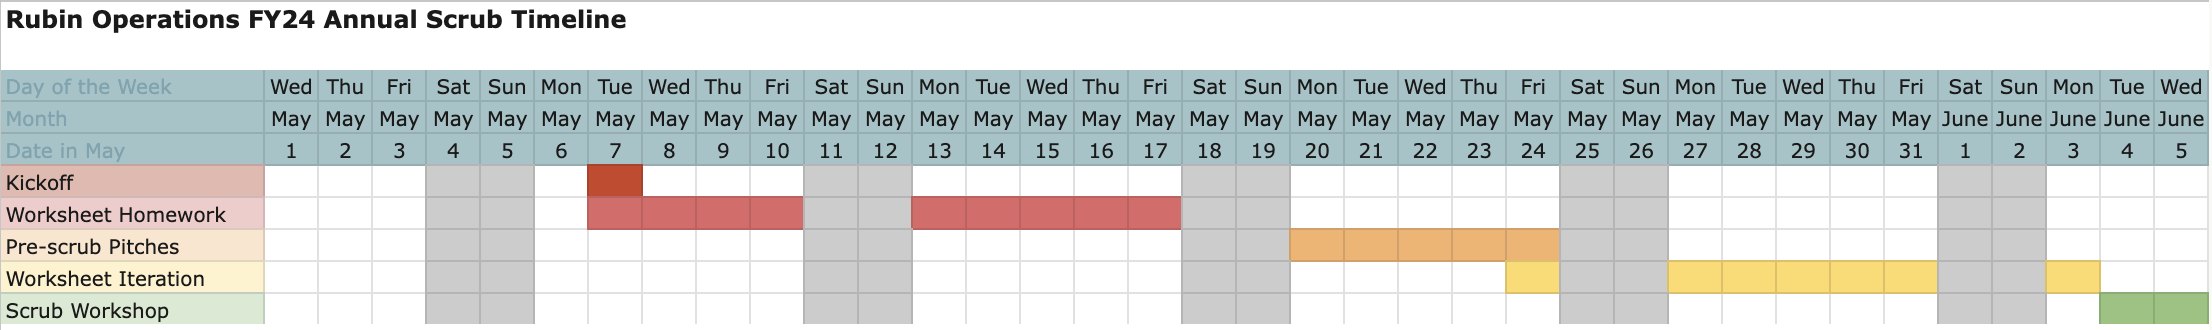
\includegraphics[width=1.0\textwidth]{Figure1Scrubtimeline}
	\caption{Scrub timeline
\label{fig:timeline}}
\end{centering}
\end{figure}
Having completed the above homework in the tool provided, the scrub moves into the ``pitches'' phase. 
Department Heads and Team Leaders prepare short presentations, for which a structured template is provided, to pitch the proposed changes to the Directors Office. 
As additional resource requests from one department could impact another, all Department Heads and Team Leaders are invited and encouraged to attend all teams' pitches, in an observatory-wide 3-day ``scrub workshop.'' 
Currently in Rubin the 15-30 minute team level pitches are presented department by department and in fully virtual format. 
This is in contrast to the US-ATLAS experiment, where the teams come together for an in-person workshop to present their proposals.
(The Rubin teams are widely distributed, geographically).

After the pitches phase is complete, a period of iteration takes place between the Directors Office and each Department/Team, in order to reach an agreement on which changes will be implemented and how.
Some compromise is needed at this point, due to budgetary constraints -- and the Team Leaders understand this, having been briefed at a virtual ``kick-off'' meeting at the start of the homework phase.

The Directors Office aggregates and costs the baseline vs proposed changes, both labor and non-labor, across the Rubin departments to ensure the program remains overall within the defined financial envelope. 
This is one of the reasons for the back and forth iterations and negotiations as priorities have to drive this process.
The aggregation is performed automatically and in real-time by the sandbox tool, so that Team Leaders and Deprtament Heads can immediately see the impact of the changes being proposed.

After agreement, the changes are implemented (by the Director's Office staff) by propagating them throughout the Rubin planning tools.
This culminates in implementation of the new spending plan for the next FY in the accounting systems at SLAC and AURA. 
Statements of Work for the next year contracts can then be generated (in July) enabling requisitions to be input in time for contracts to be placed.

With the resources now updated across all the observatory's planning tools, the teams can start realistically planning work for the coming FY by defining the tasks and activities that will lead to completion of the defined minor milestones within the boundaries of the available resources. 
Work then commences at the start of the FY. 
The work planning is done in the Atlassian tool Jira, where the milestones are defined enabling downstream and upstream traceability between milestones to tasks. 
(A full appreciation of Jira is beyond the scope of this paper.)

From the start of the FY, the Directors Office collects inputs such as overhead rates, escalation rates etc., as defined by the managing organizations, and prepares the planning tools for the next annual scrub, and so the cycle continues (see \autoref{fig:cycle}).

\begin{figure}[h!]
\begin{centering}
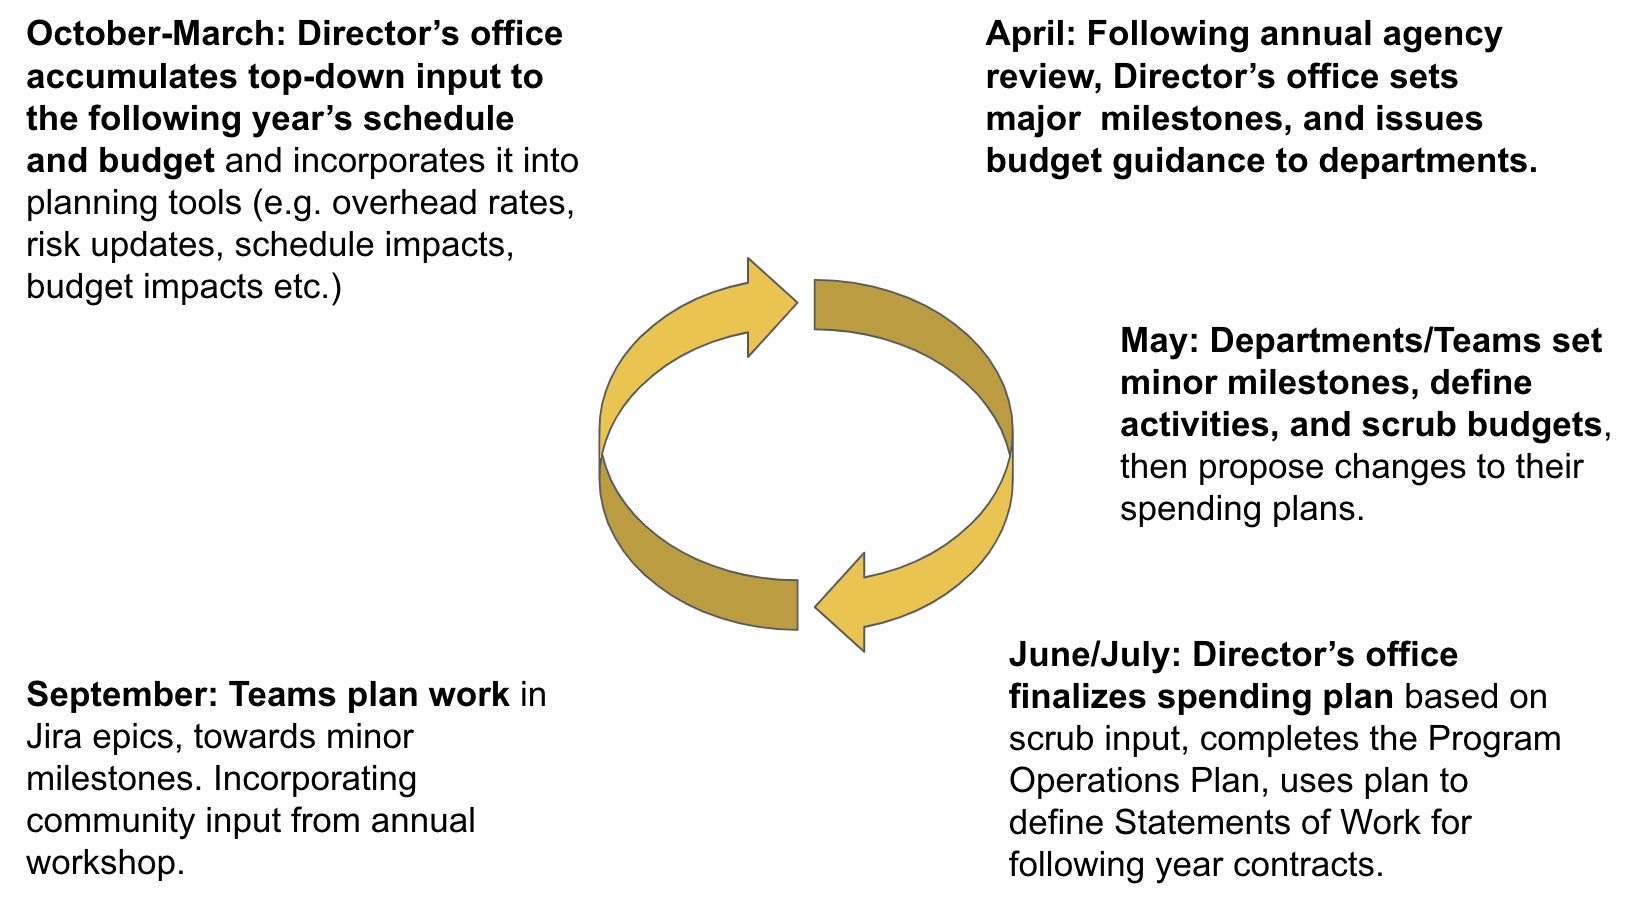
\includegraphics[width=1.0\textwidth]{Figure2AnnualPlanningScrubCycle}
	\caption{The annual planning and scrub cycle
\label{fig:cycle}}
\end{centering}
\end{figure}
